% fILE: MATH2FER.Tex
% Created: samedi 14 mai 2016, 21:37:35 (UTC+0200)

\documentclass[a4paper]{article}
\usepackage{graphics}
\usepackage[francais]{babel}
\usepackage[utf8]{inputenc}
\usepackage[T1]{fontenc}
\usepackage{listings}
\usepackage{wrapfig}
\lstset{
	basicstyle=\footnotesize,
	tabsize=3,
	language=Python
}
\begin{document}
\title{Arc de cercle pour FreeCAD}
\author{Mourad Arnout}
\maketitle
\begin{abstract}
Cet article fait partie d'un projet d'atelier menuiserie pour FreeCAD. La syntaxe de ce logiciel pour concevoir une section comprenant des rainures, des congés et des languettes est effroyablement compliquée. Les concepteurs de FreeCAD ont dû avoir du Java au biberon. 
Dans cet article on va définir un arc par un point de départ, un point d'arrivée et le vecteur tangent au premier point. 
\end{abstract}

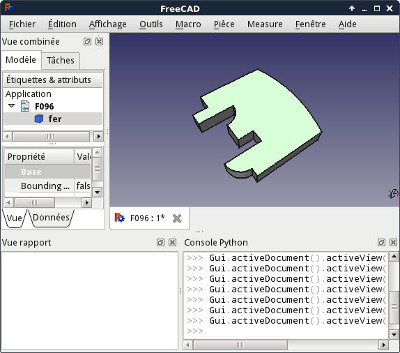
\includegraphics{../img/F096.jpg}
\newpage
\section{Coordonnées du centre de l'arc de cercle}
\begin{wrapfigure}[6]{l}{3cm}
\includegraphics{../img/arc.jpg}
\end{wrapfigure}
Il s'agit de tracer un arc de cercle partant de $ M_0 $, arrivant en $ M_1 $ et tangent \`a $ \vec{v} $ en $M_0$. Dans FreeCAD le vecteur $\vec{v}$ sera défini par son angle $a$ avec l'axe des abscisses.

Soit $ C $ le centre de ce cercle et $ I $ le milieu du segment $ [M_0 M_1] $.

Un point $ M(x, y) $ appartient \`a la droite $ (M_0 C) $ si et seulement si les vecteurs $ \overrightarrow{v}(\cos a,  \sin a) $ et $ \overrightarrow{M_0 C}(x - x_0 , y - y_0) $ sont orthogonaux :
\begin{equation}
(x - x_0)\cos a + (y - y_0)\sin a = 0  \label{eq:1}
\end{equation}

Le centre $ C $ appartient aussi \`a la m\'ediatrice de $ [M_0 , M_1] $. On en fait autant avec $ \overrightarrow{M_0 M_1} $ et $ \overrightarrow{IM} $ qui sont orthogonaux : 
\begin{equation}
(x_1 - x_0)(x - \frac{ x_0 + x_1 }{2}) + (y_1 - y_0)(y - \frac{ y_0 + y_1 }{2}) \label{eq:2}
\end{equation}
\textit{On aurait pu aussi \'ecrire que $ MM_0 ^2 = MM_1 ^2 $.}

On va maintenant arranger un peu nos affaires.
\begin{equation}
\cos a.x + \sin a.y = x_0 \cos a + y_0 \sin a \label{eq:3}
\end{equation}
\begin{equation}
(x_1 - x_0)x + (y_1 - y_0)y = \frac{x_1 ^2 - x_0 ^2 + y_1 ^2 - y_0 ^2}{2} \label{eq:4}
\end{equation}

Il ne reste plus qu'\`a r\'esoudre le syst\`eme de deux \'equations \`a deux inconnues $ x $ et $ y $. Un de mes anciens profs de physique pr\'etendait "il n'y a qu'une solution, c'est la bonne". Ici la bonne solution c'est celle des d\'eterminants que je rappellerai à la fin de cet article. On obtient aussit\^ot :
u
\begin{equation}
x = \frac{(y_1 - y_0)(x_0 \cos a + y_0 \sin a) - \frac{1}{2}(x_1 ^2 - x_0 ^2 + y_1 ^2 - y_0 ^2)\sin a}{(y_1 - y_0)\cos a - (x_1 - x_0)\sin a } \label{eq:5}
\end{equation}
\begin{equation}
y = \frac{\frac{1}{2}(x_1 ^2 - x_0 ^2 + y_1 ^2 - y_0 ^2)\cos a - (x_1 - x_0)(x_0 \cos a + y_0 \sin a)}{(y_1 - y_0)\cos a - (x_1 - x_0)\sin a}\label{eq:6}
\end{equation}

D'où le code python ci-dessous avec les notations $M_0 (x0, y0)$ $M_1 (x, y)$ et $C(X, Y)$ :

\begin{lstlisting}
	p = x*x + y*y - x0*x0 - y0*y0
	q = x0*cos(a) + y0*sin(a)
	d = (x - x0)*sin(a) - (y - y0)*cos(a)
	X = (.5*sin(a)*p - (y-y0)*q) / d # center of arc
	Y = ((x-x0)*q -.5*cos(a)*p) / d
	r = hypot(X - x, Y - y)
	a = degrees(copysign(acos((x0 - X)/r), y0 - Y))
	b = degrees(copysign(acos((x - X)/r), y - Y))
	e = Part.makeCircle(r, fv(X, Y, 0), fv(0, 0, 1), a, b)
\end{lstlisting}
\newpage
\section{Orientation du plan}
Le diable se cache dans les détails, et en math le diable c'est souvent un cauchemar d'orientation. FreeCAD trace ces arcs toujours dans le sens trigonométrique. Entre 30\degre et 45\degre il fait un petit arc, mais entre 45\degre et 30\degre il fait le grand tour. 
\begin{wrapfigure}[7]{l}{3cm}
\includegraphics{../img/sens.jpg} 
\end{wrapfigure}

Il faut donc bien lui indiquer l'angle de départ et l'angle d'arrivée. Voyez le petit dessin. Pour l'arc $M_0 M_1$ il faut lui donner en premier l'angle en $M_0$ alors que pour l'arc $M_0 M_2$ il faut donner l'angle à l'arrivée en premier. La solution miracle est le produit vectoriel $\vec{v} \wedge \overrightarrow{M_0 M_1}$. S'il est positif le sens est trigonométrique, sinon il est rétrograde. 

\bigskip
Dans notre cas simple :
\begin{equation}
\vec{v} \wedge \overrightarrow{M_0 M_1} = (0, 0, (y_1 - y_0)\cos a - (x_1 - x_0)\sin a)
\end{equation}
\bigskip
Finalement le code python de la fonction arcTo est :

\begin{lstlisting}
def arcTo(self, alpha, x, y):
	""" a is the start angle of the arc from the current point
	(x, y) is the end point
	draw an arc from the current point to (x, y)
	update the current point
	"""
	a = radians(alpha)
	x0, y0 = self.x, self.y # start point
	self.x, self.y = x, y # update current start point
	p = x*x + y*y - x0*x0 - y0*y0
	q = x0*cos(a) + y0*sin(a)
	d = (x - x0)*sin(a) - (y - y0)*cos(a)
	X = (.5*sin(a)*p - (y-y0)*q) / d # center of arc
	Y = ((x-x0)*q -.5*cos(a)*p) / d
	r = hypot(X - x, Y - y)
	g = (y - y0)*cos(a) - (x - x0)*sin(a)
	a = degrees(copysign(acos((x0 - X)/r), y0 - Y))
	b = degrees(copysign(acos((x - X)/r), y - Y))
	if g > 0:
		e = Part.makeCircle(r, fv(X, Y, 0), fv(0, 0, 1), a, b)
	else: 
		e = Part.makeCircle(r, fv(X, Y, 0), fv(0, 0, 1), b, a)
	self.addEdge(e)
\end{lstlisting}
\newpage
\section{Rappels}
\subsection{Système linéaire de deux équations à deux inconnues}

Si $ ab' - a' \not= 0 $ :
$\left\{
\begin{array}{ll}
ax + by &= c \\ 
a'x + b'y &= c' 
\end{array}
\right.$
$\Longleftrightarrow$
$\left\{
\begin{array}{ll}
x &= \displaystyle \frac{b'c - bc'}{ab' - a'b} \\
y &= \displaystyle \frac{ac' - a'c}{ab' - a'b}
\end{array}
\right.$

On se souviendra du schema opératoire ci-dessous :

\includegraphics{../img/sysdet.jpg}

\subsection{Produit vectoriel}
$ \left(\begin{array}{l}x \\y \\	z\end{array}\right) \wedge
\left(\begin{array}{l}x' \\y' \\	z'\end{array}\right) =
\left(\begin{array}{l}yz'-zy' \\zx'-xz' \\xy' - yx'\end{array}\right) 
$

\includegraphics{../img/crossvec.jpg}

\bigskip
Le produit vectoriel $\vec{u} \wedge \vec{v}$ est un vecteur $\vec{w}$  :
\begin{enumerate}
\item Orthogonal à $\vec{u}$ et à $\vec{v}$. 
\item Le trièdre $(\vec{u}, \vec{v}, \vec{w})$ est direct si et seulement si l'angle $(\vec{u}, \vec{v})$ est positif. \textit{C'est cette propriété qu'on utilise au paragraphe 2}
\item Sa norme $||\vec{w}||$ est l'aire du parallélogramme de côtés $\vec{u}$ et $\vec{v}$
\end{enumerate}
\end{document}
